\chapter{Theoretical background} \label{chap:theoreticalbackground} 

The goal of this thesis is to investigate whether the philosophy of \gls{ca}
aligns with the goals of \gls{ns}. To do so, it is essential to have a
comprehensive understanding of software stability and the key concepts, principles, and
architectures that impact software stability.

This chapter begins by examining the concepts of software stability, evolvability, and
modularity, highlighting their significance in achieving software stability in \gls{ns}.
This is followed by a brief overview of the design theorems and proposed architecture of
\gls{ns}.

The subsequent sections of the thesis explore the fundamental principles that underlie
\gls{ca}, as well as its proposed architecture designs. Finally, the thesis
concludes by discussing which aspects of \gls{ca} align with the principles of
\gls{ns} and contribute to achieving software stability in this approach.

\section{The Theoretical background of Normalized Systems} \label{ns_theory}
\begin{itemize}
    \item Inleiding
\end{itemize}


\subsection{Design Theorems of Normalized Systems} \label{subsec:ns_desing_theorems}


\subsubsection{Separation of Concerns}
\begin{itemize}
    \item Toelichting op SoC
\end{itemize}

\subsubsection{Data version transparancy}
\begin{itemize}
    \item Toelichting op data version transparancy
\end{itemize}

\subsubsection{Action version transparancy}
\begin{itemize}
    \item Toelichting op action version transparancy
\end{itemize}

\subsubsection{Separation of state}
\begin{itemize}
    \item toelichting op Separation of state.
\end{itemize}

\subsection{Construction elements}
\begin{itemize}
    \item Data elements
    \item task elements
    \item connector elements
    \item flow elements
    \item etc\dots
    \item In het hoofdstuk evaluation wordt
    besproken in hoeverre de CA construction elements convergeren met die van NS
\end{itemize}

\section{Towards stable software architectures} \label{sec:on_stability}


\gls{ns} originated in the field of software engineering, aiming to achieve modular and
stable software artifacts. However, the underlying theory of \gls{ns} can be applied to
various other domains, such as Enterprise Engineering, Business Process Modeling, and
document management. This research acknowledges the software engineering background of
gls{ns}. It consistently refers to software and Information Systems when referring to
\enquote*{artifacts}. However, the reader should realize that the concepts and artifacts
are not restricted to software artifacts alone.

In several disciplines stability has been defined as \emph{Bounded Input Bounded Output}
(BIBO). It is the fundamental property of a system when subjected to bounded input
disturbances. BIBO stability ensures that the output of a system will also be bounded,
preventing uncontrolled or unexpected behavior \parencite[270]{mannaert_normalized_2016}. 

A real-world example of the importance of stability is the Tacoma Narrows Bridge in
Washington State, USA. The bridge, depicted in figure \ref*{fig:bridge}, collapsed on
November the 7th, 1940. This was caused due to wind-induced oscillations called
aeroelastic flutter. The wind (Input) induced oscillations in the bridge, causing it to
start swaying back and forth (Output). These oscillations were initially small, but as
they continued, they began to increase in amplitude or magnitude, causing the bridge to
collapse.

\begin{figure}[H]
    \centering
    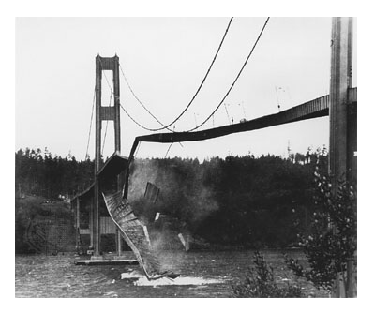
\includegraphics[width=0.6\textwidth]{Figures/bridge.pdf}
    \caption[TNB]{Tacoma Narrows Bridge (Galloping Gertie)}
    \label{fig:bridge}
\end{figure}

Stability can also be used in the context of software engineering. In the context of
\gls{ns}, it is considered a critical property that ensures that the software is not
excessively sensitive to small changes \parencite[270]{mannaert_normalized_2016}. New
functional requirements should only lead to fixed, and an expected amount of changes in
the source code. Conversely, instabilities occur when the total number of modifications
relies on the size of the software artifact. The number of changes will grow over time in
parallel with the growth of the software artifact. These instabilities are referred to as
combinatorial effects \parencite[270]{mannaert_normalized_2016}. when combinatorial effects
are absent, the software artifact can be considered evolvable.
\section{Software evolvability} \label{software_evolvability}

An important aspect of this thesis is to determine the evolvability of software artifacts
with a Clean Architecture design. An evolvable software artifact should not have
instabilities: a bounded amount of additional functional requirements cannot lead to an
unbounded amount of additional (versions of) software primitives \parencite[273]{mannaert_normalized_2009}. 

\subsection{Stability}
<<verwijzing naar positive feedback loops uit de theorie van NS en de effect op
evolueerbaarheid van software.>>

\subsection{Combinatorial effects \& anticipated change drivers.}
<<heeft relatie tot hoofdstuk evaluation en toelichtingen dat software aanpassingen niet
zouden moeten leiden tot een toename in combinatorial effects>>

\subsection{Modularity}
<<toelichten waarop modularity invloed heeft op de evolueerbaarheid van de software>>


\section{Towards evolvable software architectures} \label{sec:on_modules}

There are a couple of aspects concerning evolvable software architectures. One of which is
stability, as described in chapter \ref{sec:on_stability} \nameref{sec:on_stability}.
Another factor that impacts evolvability is the modularity of the architecture. There is a
wide consensus about two fundamental rules when thinking of-, and designing modularity:
\emph{high cohesion} and \emph{low coupling} \autocite[22]{mannaert_normalized_2016}.
These will

Software modules can be defined as self-contained units of code that perform specific
tasks or sets of tasks within a larger system. A software module is designed to operate
independently of other modules, with well-defined interfaces that allow it to communicate
and exchange data with other modules if necessary \autocite[22]{mannaert_normalized_2016}.

A module can be considered a hierarchical and recursive concept. They are independent of
their size (lines of code) or computational magnitude. They can be as small as a function
as part of a class. The class itself can also be considered a module. A group of classes
contained in a Dynamic Link Library (DLL) or Application Programming Interface (API) can
also be considered a module of an even bigger system. 

An important part of the design of a software system is to identify the possible different
modules and their interaction interfaces.

\subsection{Cohesion: The beauty of Software Desing} \label{subsec:on_modularity}

The term cohesion denotes the extent to which the various structural components of a
software system operate cohesively towards a singular and well-defined objective or goal.
Empirical studies in software engineering have extensively demonstrated the significance
of cohesion, linking higher levels of cohesion with reduced defects, enhanced
maintainability, and greater openness to change. Consequently, achieving high cohesion has
been associated with an overall improvement in software quality attributes such as
reliability, maintainability, reusability, and evolvability.

Cohesion facilitates the reduction of complexity and interdependence among the components
of a system, thereby contributing to a more efficient, maintainable, and reliable system.
By organizing components around a shared purpose or function, or by standardizing their
interfaces, data structures, and protocols, cohesion can offer the following benefits:

\begin{itemize}
    \item \textbf{Reduce redundancy and duplication of effort}: \\
    Cohesion ensures that components are arranged around a common purpose or function,
    reducing duplicates or redundant code. This simplifies system comprehension,
    maintenance, and modification.
    \item \textbf{Promoting code reuse:}\\
    Cohesion facilitates code reuse by making it easier to extract and reuse components
    designed for specific functions. This saves time and effort during development and
    enhances overall system quality.
    \item \textbf{Enhance maintainability:}\\
    Cohesion decreases the complexity and interdependence of system components, making it
    easier to identify and rectify bugs or errors in the code. This improves system
    maintainability and reduces the risk of introducing new errors during maintenance.
    \item \textbf{Increase scalability:}\\
    Cohesion improves a system's scalability by enabling it to be extended or modified
    effortlessly to accommodate changing requirements or conditions. By designing
    well-organized and well-defined components, developers can easily add or modify
    functionality as needed without disrupting the rest of the system.  
\end{itemize}

\subsection{Coupling: The beast of Software Desing} \label{subsec:on_coupling}

Coupling is a central concept in software engineering that pertains to the degree of
interdependence among software modules or components. The level of coupling between
modules denotes the strength of their relationship, whereby a high level of coupling
implies a significant degree of interdependence. Conversely, low coupling signifies a
weaker relationship between modules, where modifications in one module are less likely to
impact others.

The negative impacts of excessive coupling on software systems are considerable. High
coupling can render software systems difficult to maintain, modify, or evolve. It can
impede the identification and resolution of errors within a system, leading to prolonged
debugging periods. Additionally, it can cause fragility in the system, where slight
modifications in one module can trigger cascading failures throughout the entire system.
Therefore, it is crucial for software engineers to minimize coupling between modules while
maintaining a cohesive design. By developing systems with low coupling, software engineers
can construct more maintainable, scalable, and adaptable systems that are easier to evolve
over time.

Coupling, in software engineering, can take several forms, including content, common,
control, stamp, and data coupling. Content coupling occurs when one module accesses or
modifies the internal data or logic of another module, leading to high interdependence and
difficulty in isolating errors. Common coupling occurs when several modules access and use
the same global data, increasing their interdependence and reducing modularity. Control
coupling occurs when one module controls the execution flow of another module, making it
difficult to modify or reuse the controlled module. Stamp coupling arises when two modules
share a common data structure, leading to tight coupling and high interdependence.
Finally, data coupling exists when two modules share data, which can lead to coupling
between them.

To avoid the negative impacts of coupling on software systems, software engineers should
aim to minimize the degree of coupling between modules. This can be achieved by designing
cohesive, loosely coupled modules with well-defined interfaces. Loose coupling enables
each module to operate independently, reducing the impact of modifications made to other
modules. By implementing modular design principles, such as high cohesion and low
coupling, software engineers can develop systems that are easier to maintain, test, and
evolve.

In conclusion, coupling is a critical concept in software engineering that can have a
considerable impact on the maintainability, flexibility, and scalability of software
systems. By minimizing coupling between modules, software engineers can develop more
robust, adaptable systems that are easier to modify and evolve. Adopting modular design
principles can also facilitate the development of cohesive, loosely coupled modules that
enable the independent operation and reduce the impact of modifications made to other
modules.
\subsubsection{Cohesion} \label{subsubsec:on_cohesion}

The term cohesion denotes the extent to which the various structural components of a
software system operate cohesively towards a singular and well-defined objective or goal.
Empirical studies in software engineering have extensively demonstrated the significance
of cohesion, linking higher levels of cohesion with reduced defects, enhanced
maintainability, and greater openness to change. Consequently, achieving high cohesion has
been associated with an overall improvement in software quality attributes such as
reliability, maintainability, reusability, and evolvability.

Cohesion facilitates the reduction of complexity and interdependence among the components
of a system, thereby contributing to a more efficient, maintainable, and reliable system.
By organizing components around a shared purpose or function, or by standardizing their
interfaces, data structures, and protocols, cohesion can offer the following benefits:

\begin{itemize}
    \item \textbf{Reduce redundancy and duplication of effort}: \\
    Cohesion ensures that components are arranged around a common purpose or function,
    reducing duplicates or redundant code. This simplifies system comprehension,
    maintenance, and modification.
    \item \textbf{Promoting code reuse:}\\
    Cohesion facilitates code reuse by making it easier to extract and reuse components
    designed for specific functions. This saves time and effort during development and
    enhances overall system quality.
    \item \textbf{Enhance maintainability:}\\
    Cohesion decreases the complexity and interdependence of system components, making it
    easier to identify and rectify bugs or errors in the code. This improves system
    maintainability and reduces the risk of introducing new errors during maintenance.
    \item \textbf{Increase scalability:}\\
    Cohesion improves a system's scalability by enabling it to be extended or modified
    effortlessly to accommodate changing requirements or conditions. By designing
    well-organized and well-defined components, developers can easily add or modify
    functionality as needed without disrupting the rest of the system.  
\end{itemize}


\subsubsection{Coupling} \label{subsec:on_coupling}

Coupling is an important concept in software engineering that pertains to the degree of
interdependence among software modules and components. The level of coupling between
modules denotes the strength of their relationship, whereby a high level of coupling
implies a significant degree of interdependence. Conversely, low coupling signifies a
weaker relationship between modules, where modifications in one module are less likely to
impact others. Although not always possible, the level of coupling between the various
modules of the system should be kept to a bare minimum.

The negative impact of excessive coupling on software systems is considerable. High
coupling can render software systems difficult to maintain, modify, or evolve. It can make
it considerably more difficult to find the root cause of potential bugs. Additionally, it
causes fragility in the system, where slight modifications in one module can trigger
cascading failures throughout the entire system. Therefore, it is crucial for software
engineers to minimize coupling between modules while maintaining a cohesive design. By
developing systems with low coupling, software engineers can construct more maintainable,
scalable, and adaptable systems that are easier to evolve.

Coupling, in software engineering, can take several forms, including content, common,
control, stamp, and data coupling. Content coupling occurs when one module accesses or
modifies the internal data or logic of another module, leading to high interdependence and
difficulty in isolating errors. Common coupling occurs when several modules access and use
the same global data, increasing their interdependence and reducing modularity. Control
coupling occurs when one module controls the execution flow of another module, making it
difficult to modify or reuse the controlled module. Stamp coupling arises when two modules
share a common data structure, leading to tight coupling and high interdependence.
Finally, data coupling exists when two modules share data, which can lead to coupling
between them.

One attempt to lower coupling in the expanded artifact is to prefer stamp coupling over
data coupling through the API interface. This is done by making use of RequestModels and
ViewModels, instead of the actual data element (see example in Listings \ref{SnipModelExamples}).
Depending on the use case only the required data is passed down to the view, or in the
case of a command accepted as an input parameter.

\lstinputlisting[
    caption={The ViewModel \parencite{koks_componentviewmodel_2023} and RequestModel
    \parencite{koks_deletecomponentcommand_2023} of the Entity 'Component'
    \parencite{koks_gc_component_2023}},
    label={SnipModelExamples}]
    {Snippets/ModelExamples.cs}

\subsection{The Design Theorems} \label{subsec:ns_desing_theorems}

\gls{ns} Theorems is a theoretical framework of principles that aims to enhance the
stability of a software artifact. \gls{ns} provides a rigorous mathematical foundation
that offers guidelines for designing and developing software systems. The principles of NS
have gained significant attention in both academic and industrial circles due to their
potential to increase the evolvability and stability of software artifacts while reducing
maintenance costs. The theorems have been scientifically established and proven. In the
following sections, we will focus on the theorems of \gls{ns}. When applicable, we
emphasize some manifestations in one of the artifacts to demonstrate the level of
convergence of \gls{ca}.
\subsubsection{Separation of Concerns}

Since the early years of software engineering, \gls{soc} has been one of the fundamental
software design principles. The concept itself was introduced by
\citeauthor{parnas_criteria_1972} with his introduction of Information Hiding
\parencite{parnas_criteria_1972}. \gls{soc} as a principle has first been mentioned by
\citeauthor{dijkstra_selected_1982}\footnote{\url{https://en.wikipedia.org/wiki/Separation_of_concerns}}
as the crucial principle to design modular software architecture
\parencite[]{dijkstra_selected_1982}. 

\gls{soc} promotes the idea that a program should be divided into distinct sections, each
addressing a separate concern or aspect of a design problem. This allows for a more
organized and maintainable source code. When implemented correctly, a change to one
concern does not affect the others. \gls{soc} should be applied at the level of individual
modules, rather that the level of an entire program.

The \gls{soc} had its effect on later versions of software design principles like SOLID.
It also influenced \gls{ns}, although it has a more strict definition of this principle.
In the book of \citeauthor{mannaert_normalized_2016} it is described as followed: 

\begin{tcolorbox}
    \begin{center}
        \textbf{Theorem I}\\
        \textit{A processing function can only contain a single task to achieve stability.}    
    \end{center}        
\end{tcolorbox}

There are various manifestations of \gls{soc} observable in the artifacts. One of which is
already mentioned in Figure \ref{fig:modulair_components}, where \gls{soc} is applied to
separate the domain logic from the application, infrastructure and presentation logic.

Another example is the separation of handlers as part of the Clean Architecture Expander.
Each of those handlers executes an isolated part of the expanding process. Consider the
\citetitle{koks_expandentitieshandlerinteractor_2023}
\parencite{koks_expandentitieshandlerinteractor_2023} for example. This Handler is solely
responsible for the generation of Data Entities. 

\begin{figure}[H]
    \centering
    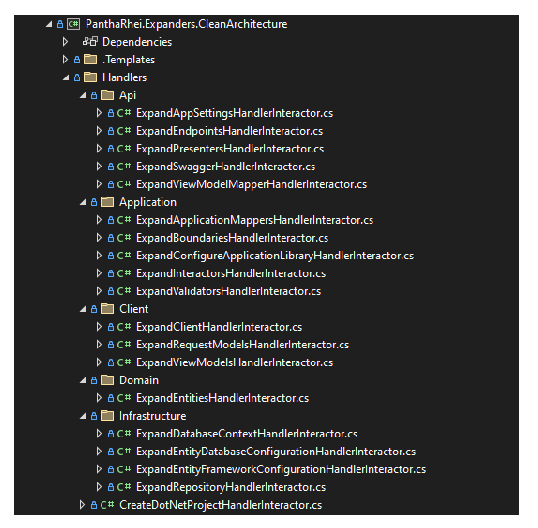
\includegraphics[width=0.8\textwidth]{Figures/expander_handlers.pdf}
    \caption[handlers]{Each of the handlers handles an isolated part of the expanding process.}
    \label{fig:handlers}
\end{figure}
\subsubsection{Data version Transparancy}

\gls{dvt} is the act of encapsulation of data entities for specific tasks at hand. This
results in the fact that data structures can have multiple versions often mentioned as
Data Transfer Objects in modern software engineering projects. In other words, it should
be possible to update the data entity without affecting the processing functions. This
leads to the following description of the theorem \parencite[280]{mannaert_normalized_2016}.

\begin{tcolorbox}
    \begin{center}
        \textbf{Theorem II}\\
        \textit{A data structure that is passed through the interface of a processing function 
        needs to exhibit version transparency in order to achieve stability.}
    \end{center}    
\end{tcolorbox}

\gls{dvt} is widely used in various technological applications. practically every web
service currently known supports some type of versioning. In restful APIs for example, it
is common practice to support versioning over the URI. It is considered a best practice
to encapsulate breaking changes in a new version of the endpoint/service so that the
consumers are not (directly) affected by the change. In modern Object Oriented languages,
gls{dtv} is also supported by the ability to determine the scope of visibility of the
modifiers of the various programming constructs like fields, properties, interfaces and
classes. Also known as information hiding
\parencites{parnas_criteria_1972}[278]{mannaert_normalized_2016}.

The prototype also uses information hiding very strictly. In order to seal implementations
to the intended layers, concrete implementations always have internal visibility, making
them impossible to use. The interfaces on the other hand are publically exposed. The
dependent layers are now restricted to the appointed dependency injection container of the
specific layer. Alternatively, it is also possible to implement a custom implementation of
the specific interface. 

Another example from the prototype is the use of ViewModels for the queries, and
CommandModels for the commands. Depending on the context of the operation, the containing
fields of the Model may differ. A CommandModel for deleting a data entity will only
contain the key of the entity that needs to be deleted. The CommandModel for creating the
same type of entity will probably contain all the required fields of the data entities,
except the key field as this key is often auto-generated by the database or
domain layer of the application.
\subsubsection*{Action version Transparancy}
\gls{avt} is the property of a system to modify existing processing functions without
affecting the existing ones. It should be possible to upgrade a function without affecting
the callers of those functions. This description leads to the following theorem
\parencite[282]{mannaert_normalized_2016}.

\begin{tcolorbox}[boxrule=0.1pt, colback=mygray, title=Theorem III,colbacktitle=gray]
    \textit{A processing function that is called by another processing function, needs to exhibit version transparency in order to achieve stability.}
\end{tcolorbox}

Most of the modern technology environments support some form of \gls{avt}. Polymorphism is
a widely used technique in order to support this theorem. Specifically, parametric
polymorphism \footnote{\url{https://en.wikipedia.org/wiki/Parametric_polymorphism}} allows
for a processing function to have multiple input parameters. There are also quite some
design patterns supporting this theorem. Some random examples are the state pattern
\footnote{\url{https://en.wikipedia.org/wiki/State_pattern}}, facade pattern
\footnote{\url{https://en.wikipedia.org/wiki/Facade_pattern}} and observer pattern
\footnote{\url{https://en.wikipedia.org/wiki/Observer_pattern}}.
\subsubsection{Separation of State}

\gls{sos} is a theorem that is based on the idea that processing functions should not
contain any state information but instead should rely on external data structures to store
state information. By separating state information from processing functions, Normalized
Systems can achieve a higher level of flexibility and adaptability. External data
structures can be updated or replaced without affecting the processing functions
themselves, which greatly reduces the change of unwanted ripple effects. This theorem is
described as followed: \parencite[258]{mannaert_normalized_2016}.

\begin{center}
    \textbf{Theorem IV}\\
    \textit{Calling a processing function within another processing function, needs to exhibit state keeping in order to achieve stability.}
\end{center}

\gls{sos} fits very well in distributed information systems with asynchronous calls. The
expanded artifact is designed in a manner that all external process functions are executed
asynchronously. \todo{snippet toevoegen.}.

A simpler manifestation of the \gls{sos} theorem involves the use of Resources as an
integral part solution
\footnote{url{https://learn.microsoft.com/en-us/dotnet/core/extensions/resources}}. In
addition to enabling the localization of strings, this approach offers the advantage of
centralized management, thereby exhibiting \gls{sos}. For instance, when the functional
requirements evolve, the name of a template in the expander artifact is likely to change.
As the name of the template is used in multiple class instances, a centralized approach to
managing the template name can mitigate the risk of excessive modifications when a name
change is mandated.

Another example. The state of the model (see chapter \ref{sec:artifact_model}) is
currently persisted in an Azure SQL Database.

\lstinputlisting[
    caption={The \citetitle{koks_genericrepository_2023} \parencite{koks_genericrepository_2023}}]
    {Snippets/GenericRepository.cs}

The state of of the expander artifact model as described in \ref{sec:artifact_model} for the expander in the 
voorbeeld met seerders...
voorbeeld met repositories....
\subsection{On the emergence of element} \label{subsec:ns_elements} 

\textbf{Data Element}\\
This is an object that represents a piece of data in the system. Data elements are used to
pass information between processing functions and other objects. In Normalized Systems,
data elements are typically standardized to ensure consistency across the system.

\textbf{Flow Element}\\
This object represents the flow of control through the system. It determines the order in
which processing functions are executed and can be used to handle error conditions or
other exceptional cases.

\textbf{Connector Element}\\
This object is used to connect different parts of the system together. Connectors can be
used to link processing functions, data elements, and other objects, allowing them to work
together seamlessly.

\textbf{Task Element}\\
This is an object that represents a specific task or action in the system. Tasks can be
composed of one or more processing functions and can be used to represent complex
operations within the system.

\section*{The Theoretical background of Clean architecture}

\subsection*{Introduction}
